\begin{titlepage}

\begin{center}

% Oberer Teil der Titelseite:
%\includegraphics[width=0.15\textwidth]{./logo}\\[1cm]    
\textsc{\LARGE Produktentwicklung 2}\\[1.5cm]

\textsc{\Large Hochschule Luzern\\
    ~\\
    Technik \& Architektur}\\[0.5cm]

\vfill{}

% Title
\newcommand{\HRule}{\rule{\linewidth}{0.5mm}}
\HRule \\[0.4cm]
{   \Huge \bfseries Projektplanung\\
        ~\\
        \large Einführung in die Projektverwaltung mit GitHub}\\[0.4cm]

\HRule \\[1.5cm]

% Author and supervisor
\begin{minipage}{0.4\textwidth}
    \begin{flushleft} \large
        \emph{Autoren:}\\
        \textsc{Pren Team 39}\\
        Adriano \textsc{Valsangiacomo}\\
        Christian \textsc{Spycher}\\
        Christian \textsc{Schürch}\\
        Ervin \textsc{Mazlagi\'c}\\
        Fabian \textsc{Wüthrich}\\
        Alexander \textsc{Suter}\\
	Adrian \textsc{Würsch}
    \end{flushleft}
\end{minipage}
\hfill
\begin{minipage}{0.4\textwidth}
    \begin{flushright} \large
        \emph{Modulbetreuer:} \\
        Martin \textsc{Vogel}
    \end{flushright}
\end{minipage}

\vfill{}
\vfill{}
\vfill{}

% Unterer Teil der Seite
{\large Horw\\ \today}

\end{center}

\end{titlepage}
		% Titelseite
\thispagestyle{empty}

\begin{abstract}
Die erfolgreiche Realisierung eines Projektes verlangt nach einer
gewissen Struktur und Organisation. Diese liegen insbesondere im
Bereich der Planung und kontinuierlichen Kontrolle. Als Elementare
Intrumente gehören hierzu nach klassischen Modellen des
Projektmanagments die Meilensteine und Arbeitspakete.

In der vorligenden Arbeit soll zunächt eine kurze Einführung in die
theoretischen Aspekte dieser Instrumente gegeben werden. In einem 
weiteren Abschnitt wird die Methode des kollaborativen
Projemtmanagements soweit erläutert, wie es für die Verknüpfung für
die Verwendung mit GitHub notwendig ist. Die Beschreibung der
praktischen Umsetzung und der dazu eingesetzten Mittel stellt den
letzten Abschnitt der Arbeit dar, welcher auch einige Beispiele aus
der Umsetzung aufzeigt und Hinweise für die Verwendung gibt.
\end{abstract}
	% Abstract
\newpage
\tableofcontents		% Inhaltsverzeichnis
\newpage

%Beschreibung des Lösungskonzepts
\section{Management Summary}
Die vorliegende Dokumentation befasst sich mit der Umsetzung des Lösungskonzepts der Gruppe 39 für eine autonome Ballwurfmaschine.
Im Rahmen des Moduls PREN2 setzen wir uns mit dem Zusammenbau und dem Testen des Prototypen und dessen Funktionen auseinander.
Dazu wurden die Komponenten eingekauft und wenn notwendig angepasst. Von der Elektrotechnik wurden sämtliche Boards und Steuerungen bereitgestellt.
So kann die Informatik über bestimmte Schnittstellen optimal auf die Maschine zugreifen und diese steuern.
\newpage
\section{Einleitung}

Suchen, anvisieren und treffen. Zu Urzeiten waren diese Tätigkeiten überlebensnotwendig, wollte man etwas Fleisch zwischen die Zähne bekommen. Einige Zeitalter später steht man beinahe vor der gleichen Problemstellung. Jedoch soll kein Blut fliessen. Denn das Ziel ist kein lebendiges Tier sondern ein schwarzer, feststehender Korb. Dieser Korb muss gefunden werden, die Ausrichtung muss diesen anvisieren und schlussendlich müssen fünf Tennisbälle hinein befördert werden.

In der Aufgabenstellung wurde eine Ballwurfmaschine gefordert, welche nach einem Startsignal, selbständig den Korb findet und die Bälle hinein befördert. Das PREN Team 39 hat in einer ersten Phase ein Konzept für eine solche Maschine erarbeitet. Es wurden verschiedene Lösungsansätze verfolgt und nach einem einheitlichen Raster bewertet. Die Idee mit der höchsten Punktzahl wurde im Detail ausgearbeitet um diese schlussendlich in der zweiten Phase umzusetzen. Angehende Maschinenbau-, Elektrotechnik- und Informatik-Ingenieure setzten sich zusammen um das Konzept optimal umzusetzen. Die Interdisziplinarität spielt eine grosse Rolle und ist ein wesentlicher Bestandteil des Projekts.

In der vorliegenden Arbeit wird zuerst grob auf das Lösungskonzept eingegangen. Anschliessend werden in den einzelnen Disziplinen die Komponenten beschrieben. Der mechanische Aufbau, die Verkabelung der Elektrotechnik sowie die Architektur der Software sind festgehalten. Informationen zum Projektmanagement wie die Organisation, die Planung, die Kosten und das Risikomanagement liegen nachfolgend vor. Detaillierte Informationen sind im Anhang vorhanden.



\newpage
\subsection{Produktbeschreibung}
\subsection{Übersichtszeichnung}
Die Ballwurfmaschine funktioniert nach einem einfachen Konzept. Der Ball wird in eine Verengung geschoben und durch ein Drehrad nach vorne gedrückt. Dadurch wird er beschleunigt und zielgerichtet auf seine Flugbahn gelenkt.
\begin{figure}[h!]
	\centering
	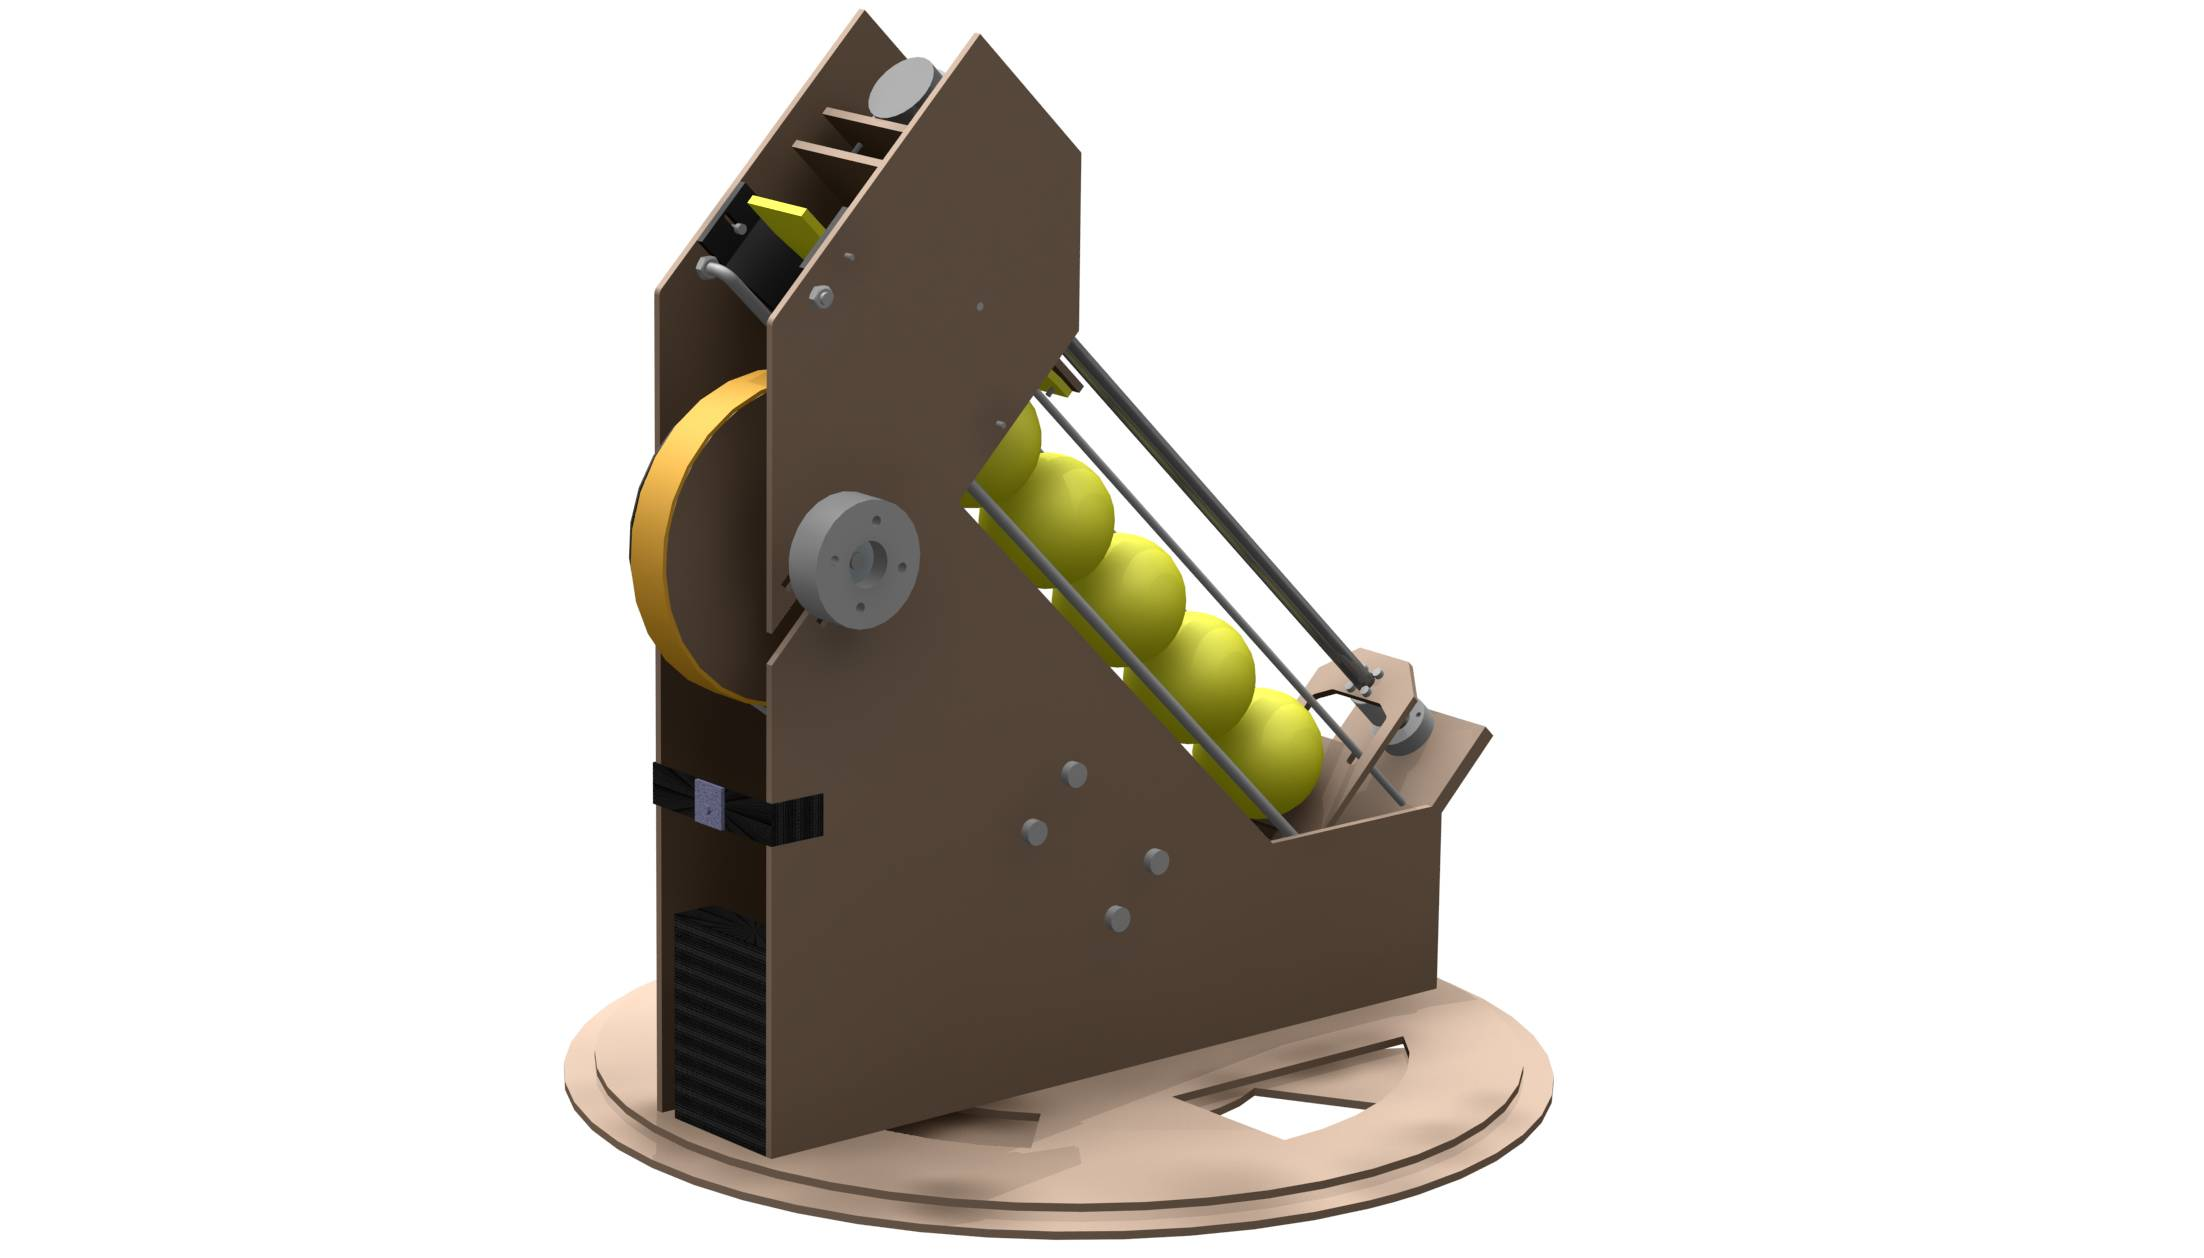
\includegraphics[width=\linewidth]{../../fig/Render_Komplettsystem}
	\caption{Übersichtszeichnung}
	\label{fig:Übersichtszeichnung}
\end{figure}
\newpage
\subsubsection{Blockdiagramm}
Das Blockdiagramm beschreibt den Zusammenhang der einzelnen Komponenten. In Abbildung \ref{fig:blockdiagramm} wird dies dargestellt. Die externe Steuerungseinheit (Notebook) greift über WLAN auf das Raspberry Pi zu. Dieses kommuniziert mit der PI-Kamera für die Detektion des Korbes. Zudem greift das Pi auf das Freedom Board zu, welches wiederum zuständig für alle Motoren ist. Die Turmausrichtung übernimmt der Stepper, die Beschleunigung des Schwungrades ist Sache des BLDC-Motors und für den Ballnachschub ist der DC-Motor zuständig.

\begin{figure}[h!]
\centering
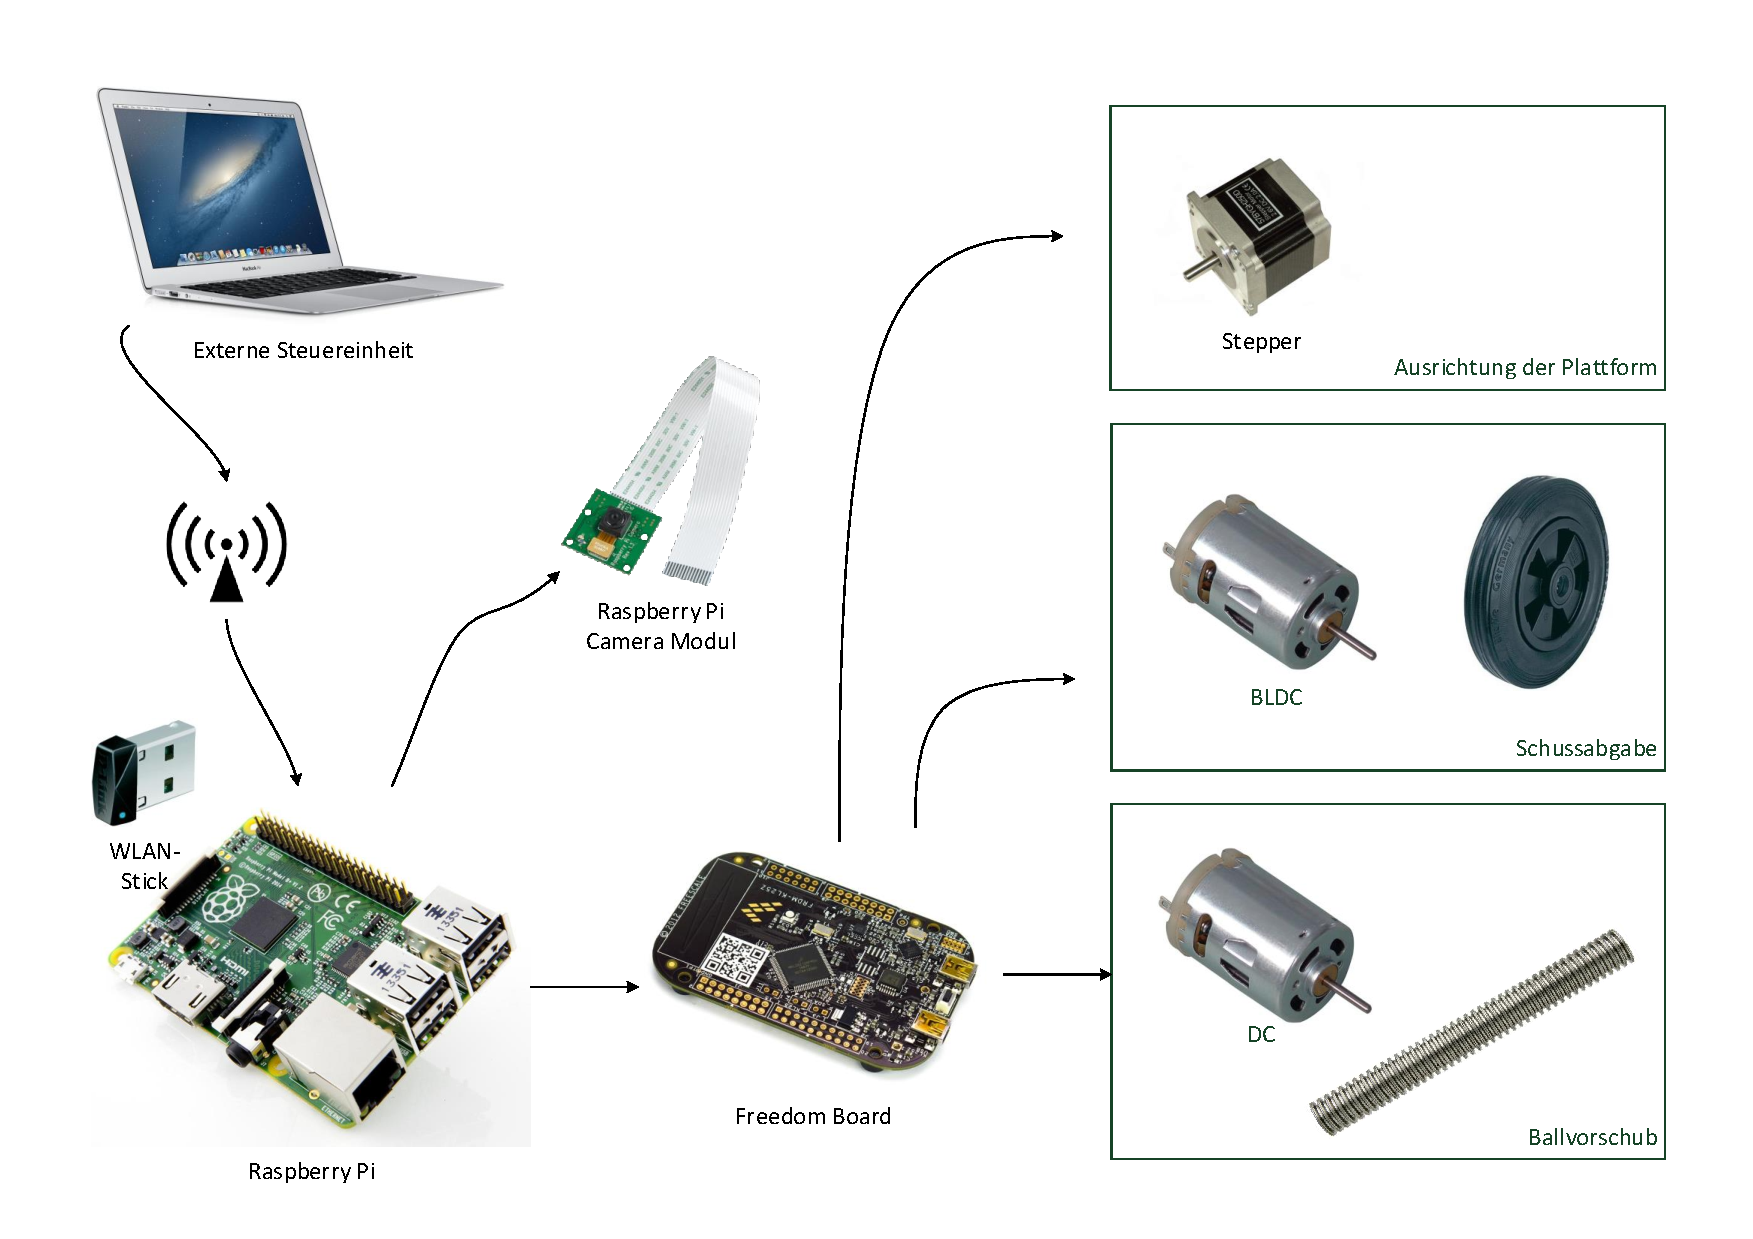
\includegraphics[width=0.9\linewidth]{../../fig/blockdiagramm}
\caption{Blockdiagramm}
\label{fig:blockdiagramm}
\end{figure}

\newpage
\subsubsection{Ablaufdiagramm}
Der allgemeine Ablauf der autonomen Wurfmaschine kann als endlicher Automat
modelliert werden, denn es gibt einen definierten Einstiegs- und 
Ausstiegspunkt. Der Einstieg (Start) ist definiert durch den Beginn der 5 minütigen Kalibrierung und der Ausstiegspunkt (Ende) ist gegeben, wenn der Ballvorschub den vorderen Endpunkt erreicht hat. Zwischen Start und Ende muss das Zielobjekt identifiziert, die Maschine ausgerichtet, die Wurfautomatik parametriert und schlussendlich der Wurf durchgeführt werden.

\begin{figure}[h!]
	\centering
	\begin{tikzpicture}[shorten >=2pt,node distance=4cm,on grid,auto]
	\node[state,initial] 	(q_0) 						{$q_0$};
	\node[state] 			(q_1) [above=of q_0]		{$q_1$};
	\node[state]			(q_2) [right=of q_1]		{$q_2$};
	\node[state]			(q_3) [right=of q_2]		{$q_3$};
	\node[state]			(q_4) [right=of q_3]		{$q_4$};
	\node[state,accepting]	(q_5) [below=of q_4]		{$q_5$};
	\path[->]
	(q_0)	edge node	{\begin{tabular}{c} Startsignal \end{tabular}} (q_1)
	(q_1)	edge node	{Korb entdeckt}	(q_2)
	(q_2)	edge node	{\begin{tabular}{c} Plattform \\ ausgerichtet \end{tabular}}	(q_3)
	(q_3)	edge node	{Drehzahl erreicht}	(q_4)
	(q_4)	edge node	{\begin{tabular}{c} Keine Bälle \\ vorhanden \end{tabular}}	(q_5);
	\end{tikzpicture}
	\caption{Autonome Wurfmaschine modelliert als endlicher Automat}
\end{figure}

\noindent
\textbf{Zustands- und Zustandsübergangsbeschreibungen}
\begin{itemize}
	
	\item Start \\ \\
	Gestartet wird nicht mit dem eigentlichen autonomen Prozess, sondern mit der Einrichtung der Maschine und der Kalibrierung.
	
	\item Kalibrierung ($q_{0}$) \\ \\
	Zu Beginn steht eine 5 minütige Kalibrierung zur Verfügung. In dieser Phase kann die Elektronik auf die Mechanik abgestimmt und allfällige Einstellungen am Bildverarbeitungssystem vorgenommen werden. Nach Ablauf dieser 5 Minuten darf keine Änderung am System mehr vorgenommen werden. Siehe dazu Anhang \ref{fig:ablauf-ballwurf}.
	
	\item Zustandsübergang von $q_{0}$ zu $q_{1}$ \\ \\
	Der eigentliche Prozess erfolgt nun mittels eines Start-Signales, welches von einer externen Steuerungseinheit drahtlos übermittelt wird.
	
	\item Ortung des Korbs ($q_{1}$) \\ \\
	Zur Ortung des Korbs wird ein Foto mit einer eingebauten Kamera gemacht. Dieses Foto wird mittels eines eigenen Algorithmus ausgewertet um den Ort zu bestimmen. Der Korb wird immer entdeckt, was jedoch nicht automatisch bedeutet, dass die richtige Position zurückgegeben wird. Denn statt das System stillzulegen, wenn der Korb nicht detektiert wird, kann man immer noch auf Basis des Zufalls erfolgreich sein.
	
	\newpage
	
	\item Zustandsübergang von $q_{1}$ zu $q_{2}$ \\ \\
	Sobald die Detektierung abgeschlossen ist, wird der einzustellende Winkel der Komponente, welche für die Ausrichtung zuständig ist, übermittelt.
	
	\item Plattform ausrichten ($q_{2}$) \\ \\
	Die Plattform wird anhand der Positionsdaten ausgerichtet.
	
	\item Zustandsübergang von $q_{2}$ zu $q_{3}$ \\ \\
	Sobald der Prozess zur Ausrichtung der Plattform vollzogen ist, wird in den nächsten Zustand gewechselt.
	
	\item Drehzahl erreichen ($q_{3}$) \\ \\
	Der Antrieb des Drehrades wird gestartet. Damit immer von den gleichen Anfangsbedingungen ausgegangen werden kann, muss zuerst eine vorher definierte Drehzahl erreicht werden. Es wird die Anlaufverzögerung des Motors abgewartet und gemessen ob die gewünschte Drehzahl erreicht wurde.
	
	\item Zustandsübergang von $q_{3}$ zu $q_{4}$ \\ \\
	Sobald die Soll-Drehzahl erreicht wurde, wird in den nächsten Zustand gewechselt. Die Drehzahl wird bis zum Ende des ganzen Abwurfs konstant bleiben. Es wird darauf verzichtet, das Rad nach jedem Wurf zu stoppen und wieder neu zu starten.
	
	\item Ballvorschub starten ($q_{4}$) \\ \\
	Die Ballwurfmaschine ist somit schussbereit. Als nächstes wird der Spindelantrieb des Ballvorschubes gestartet. Der Ballvorschub führt die Bälle an das Drehrad heran und die Bälle werden beschleunigt. 
	
	\item Zustandsübergang von $q_{4}$ zu $q_{5}$ \\ \\
	Sobald der Ballvorschub den vorderen Endpunkt erreicht hat, wurden alle Bälle abgeworfen und es kann in den nächsten Zustand gewechselt werden.
	
	\item Stoppsignal senden ($q_{5}$) \\ \\
	Die externe Steuerungseinheit, welche das Start-Signal abgegeben hat, erhält das Stoppsignal.
	
	\item Ende \\ \\
	Mit dem Erhalt des Stoppsignal ist der Prozess abgeschlossen.
	
\end{itemize}

\noindent
\textbf{Fehler-Szenarien}
Während des ganzen Ablaufs können Fehler auftreten. Fällt eine Teilfunktion aus, so soll nach Möglichkeit trotzdem immer in den nächsten Zustand gewechselt werden. Kann beispielsweise der Korb nicht detektiert werden, so soll ein Zufallswinkel dem nächsten Zustand übermittelt werden. Kann die Plattform nicht ausgerichtet werden, dann soll die Transition in den nächsten Zustand trotzdem erfolgen. Wird nicht die gewünschte Drehzahl erreicht, soll anschliessend trotzdem versucht werden die Bälle abzuschiessen. Das Motto bei einem Fehler ist somit immer Best-Effort. Es ist nicht nötig direkt in den $q_{5}$ zu wechseln. Jede Funktion kann trotzdem ausgeführt werden, wenn eine davor liegende Funktion nicht ausgeführt werden konnte.

\newpage
\newpage
\subsection{Übersichtszeichnung}
Die Ballwurfmaschine funktioniert nach einem einfachen Konzept. Der Ball wird in eine Verengung geschoben und durch ein Drehrad nach vorne gedrückt. Dadurch wird er beschleunigt und zielgerichtet auf seine Flugbahn gelenkt.
\begin{figure}[h!]
	\centering
	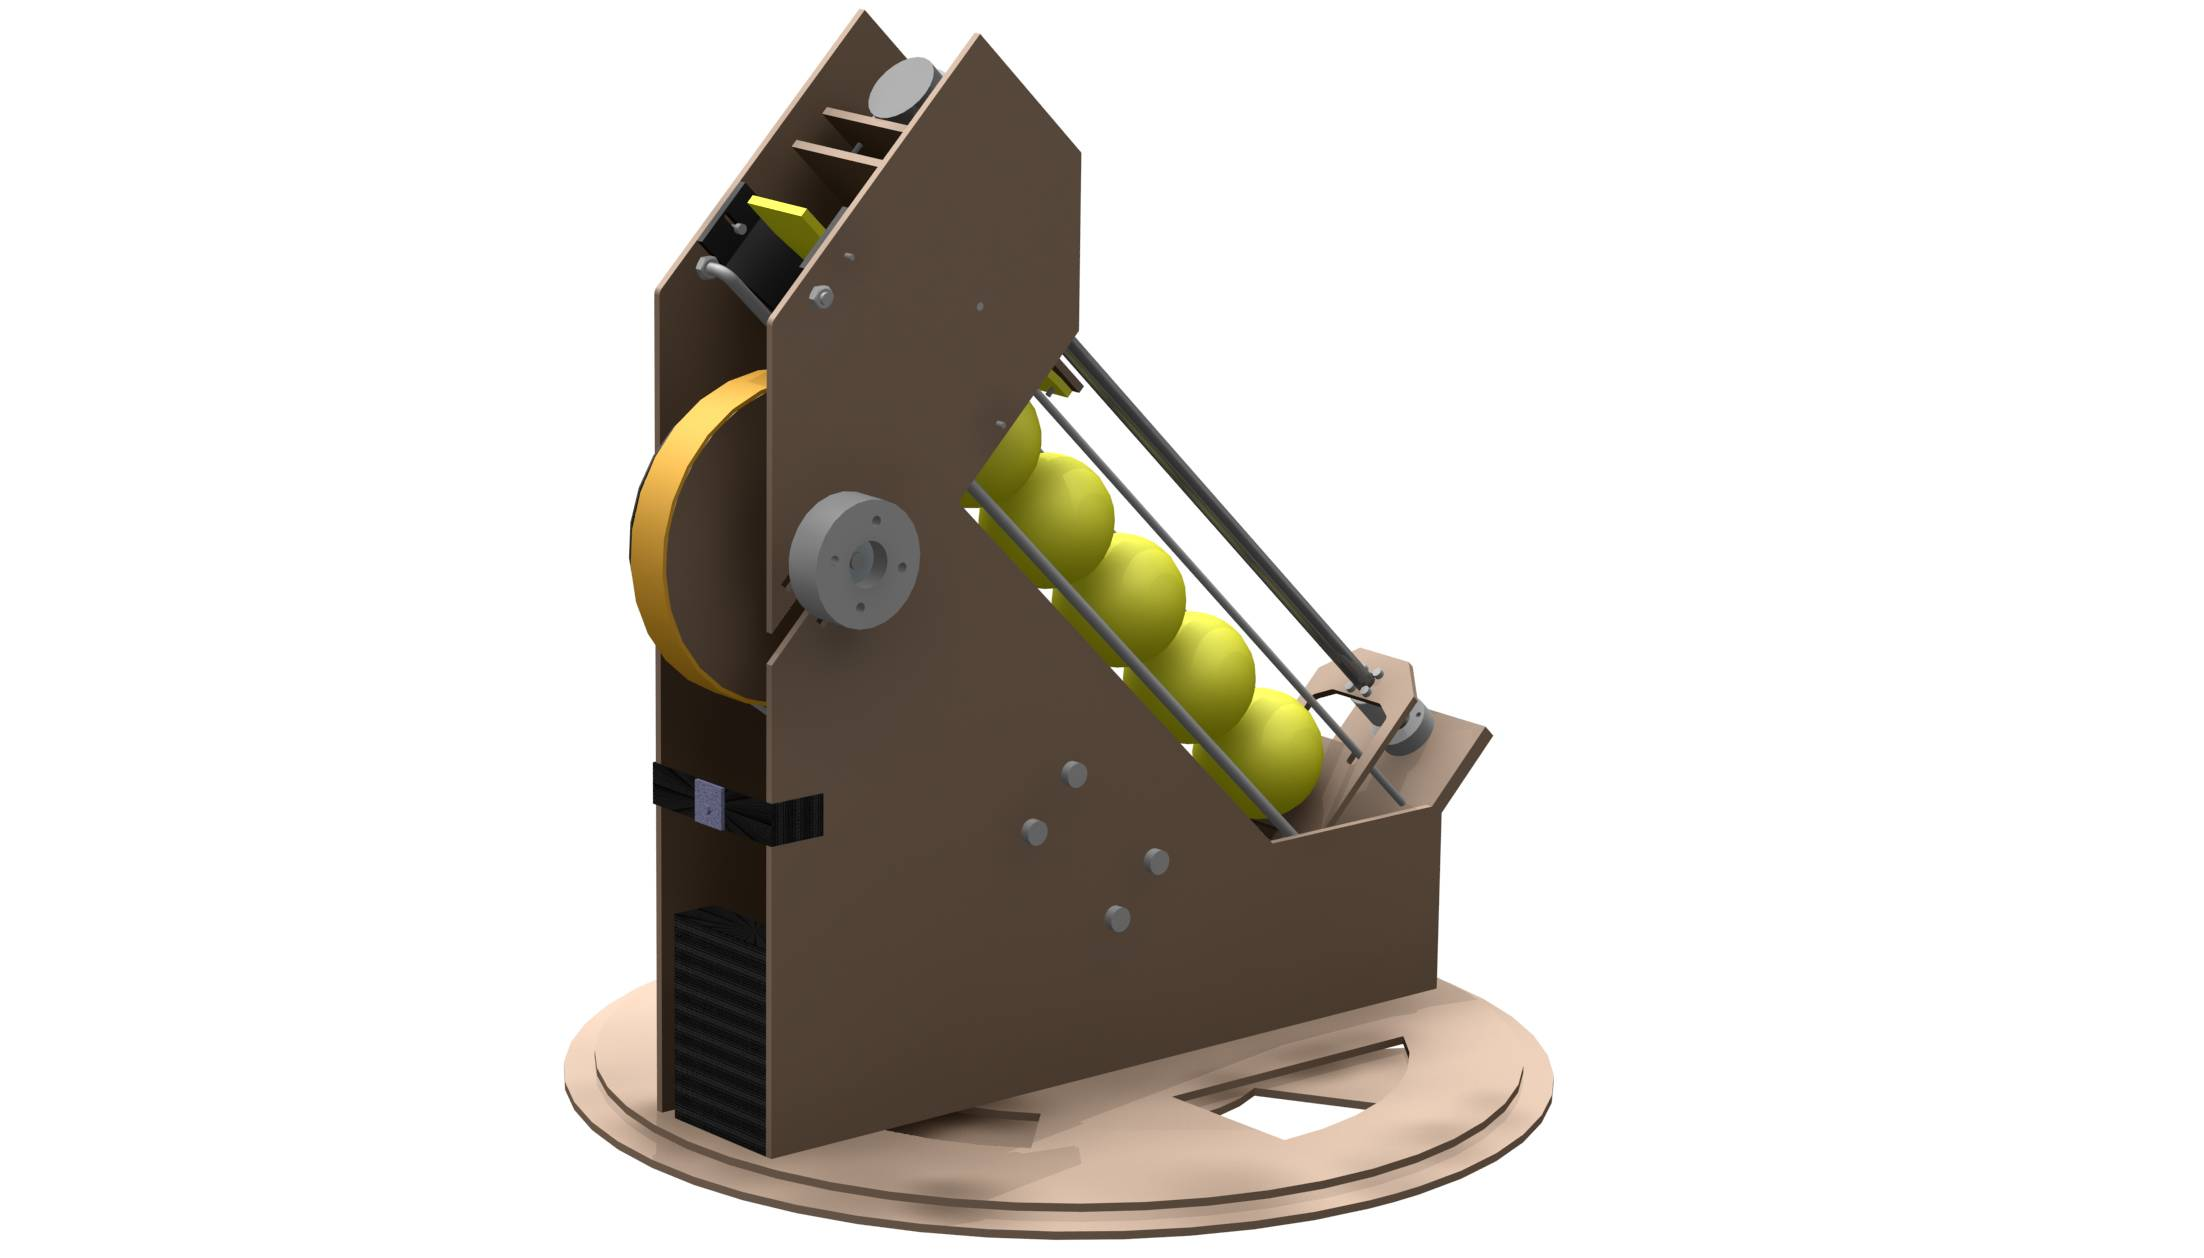
\includegraphics[width=\linewidth]{../../fig/Render_Komplettsystem}
	\caption{Übersichtszeichnung}
	\label{fig:Übersichtszeichnung}
\end{figure}
\newpage
\input{content/komponenten}
\newpage
\input{content/ablaufdiagramme}
\newpage
\input{content/funktionalitaet}
\newpage
\section{Schnittstellen}

\section{REST von Webserver}

Die Schnittstelle von der externen Steuereinheit zum Raspberry Pi wird über eine REST\footnote{Representational State Transfer}-Schnittstelle realisiert. Es wurden folgende Ressourcen definiert:
\begin{itemize}
	\item camera
	\item image
	\item start
\end{itemize}
Jede Ressource lässt sich mit HTML-Methoden (GET, PUT, POST usw.) abrufen oder verändern. Die Schnittstelle lässt sich ohne Authentifizierung nutzen und arbeiten mit dem JSON-Datenformat. Nachfolgend werden die einzelnen Ressourcen näher beschrieben.

\subsection{GET camera}

Diese Anfrage liefert die aktuellen Einstellungen der Bilderkennung zurück.

\subsubsection{Parameter}

\begin{tabular}{l p{16cm}}
	\textbf{config} & Die Konfiguration der Bilderkennung \\
	\textbf{roi} & Ist der Bereich in dem der Korb erkennbar ist (Region of Interest). Er ist definiert durch die Koordinaten der linken oberen Ecke (x,y) und einer Fläche (height, width). \\
	\textbf{contrast} & Ein Wert zwischen -100 und 100 für den Kontrast der Kamera. \\
	\textbf{greyscale} & \texttt{true} wenn ein Graustufen-Bild erzeugt werden soll. \\
	\textbf{quality} & Ein Wert zwischen 0 und 100 für die Qualität des JPEG-Bildes. \\
	\textbf{line} & Die Pixellinie welche analysiert werden soll um den Korb zu detektieren. \\
	\textbf{height} & Auf welcher Höhe soll die Pixellinie analysiert werden. Darf max. so hoch sein wie die ROI. \\
	\textbf{area} & Bei der Detektierung wird nicht nur eine Pixellinie untersucht. Mit \texttt{area} kann ein Band definiert werden in dem die Linien analysiert werden. \\
	\textbf{image} & Der URL zum Bild der Kamera. Bei jedem Aufruf wird ein neues Bild erstellt.
\end{tabular}

\subsubsection{Beispiel Request}

\texttt{GET} \\
\texttt{http://<raspberrypi-ip>/camera}

\subsubsection{Beispiel Result}

\begin{lstlisting}[caption=GET camera Result, label=lst:camera, tabsize=2]
{
	"config": {
		"roi": {
			"x": 100,
			"y": 200,
			"height": 300,
			"width": 400
		},
		"contrast": 50,
		"greyscale": true,
		"quality": 100,
		"line": {
			"height": 300,
			"area": 5
		}
	},
	"image": "http://<raspberrypi-ip>/image"
}
\end{lstlisting}

\subsection{PUT camera}

Diese Anfrage verändert die Einstellungen der Bilderkennung.

\subsubsection{Beispiel Request}

\texttt{PUT} \\
\texttt{http://<raspberrypi-ip>/camera} \\
Body siehe Listing \ref{lst:camera}

\subsubsection{Beispiel Result}

\begin{lstlisting}[caption=PUT camera Result, tabsize=2]
{
	"status": true
}
\end{lstlisting}

\subsection{GET image}

Diese Anfrage liefert das Bild der Kamera zurück. Bei jeder Anfrage wird ein Bild erstellt.

\subsubsection{Beispiel Request}

\texttt{GET} \\
\texttt{http://<raspberrypi-ip>/image}

\subsubsection{Beispiel Result}

Bild im JPEG-Format

\subsection{GET start}

Diese Anfrage liefert den Status des Vorgangs zurück. Wenn \texttt{start} auf \texttt{true} gesetzt ist läuft der Vorgang.

\subsubsection{Beispiel Request}

\texttt{GET} \\
\texttt{http://<raspberrypi-ip>/start}

\subsubsection{Beispiel Result}

\begin{lstlisting}[caption=GET start Result, tabsize=2]
{
	"start": true
}
\end{lstlisting}

\subsection{PUT start}

Diese Anfrage startet den Vorgang und übergibt die Callback-Adresse vom Steuergerät, damit der Stopp-Befehl zurück gesendet werden kann.

\subsubsection{Parameter}

\begin{tabular}{l p{16cm}}
	\textbf{start} & Bei \texttt{true} wird der Vorgang gestartet. Der Vorgang wird nicht unterbrochen falls \texttt{start} auf \texttt{false} gesetzt wird. Ist der Vorgang beendet wird \texttt{start} auf \texttt{false} gesetzt \\
	\textbf{url} & Die IP-Adresse des Steuergerätes. Diese wird benötigt um den Stopp-Befehl zurückzusenden.
\end{tabular}

\subsubsection{Beispiel Request}

\texttt{PUT} \\
\texttt{http://<raspberrypi-ip>/start}

\begin{lstlisting}[caption=PUT start Request, tabsize=2]
{
	"start": true,
	"url": "http://<steuergerät-ip>"
}
\end{lstlisting}

\subsubsection{Beispiel Result}

\begin{lstlisting}[caption=PUT start Result, tabsize=2]
{
	"status": true
}
\end{lstlisting}
\newpage
\input{content/softwaresubsysteme}
\newpage
\input{content/berechnungen}
\newpage
\input{content/versuche-tests}
\newpage
%Projektmanagement und Projektplanung
\input{content/projektmanagement-planung}
\newpage
%Schlussdiskussion mit den Unterabschnitten
\input{content/entwicklungskosten}
\newpage
\input{content/lessons-learned}
\newpage

%Anhang
\appendix
\section{Aufgabenstellung}

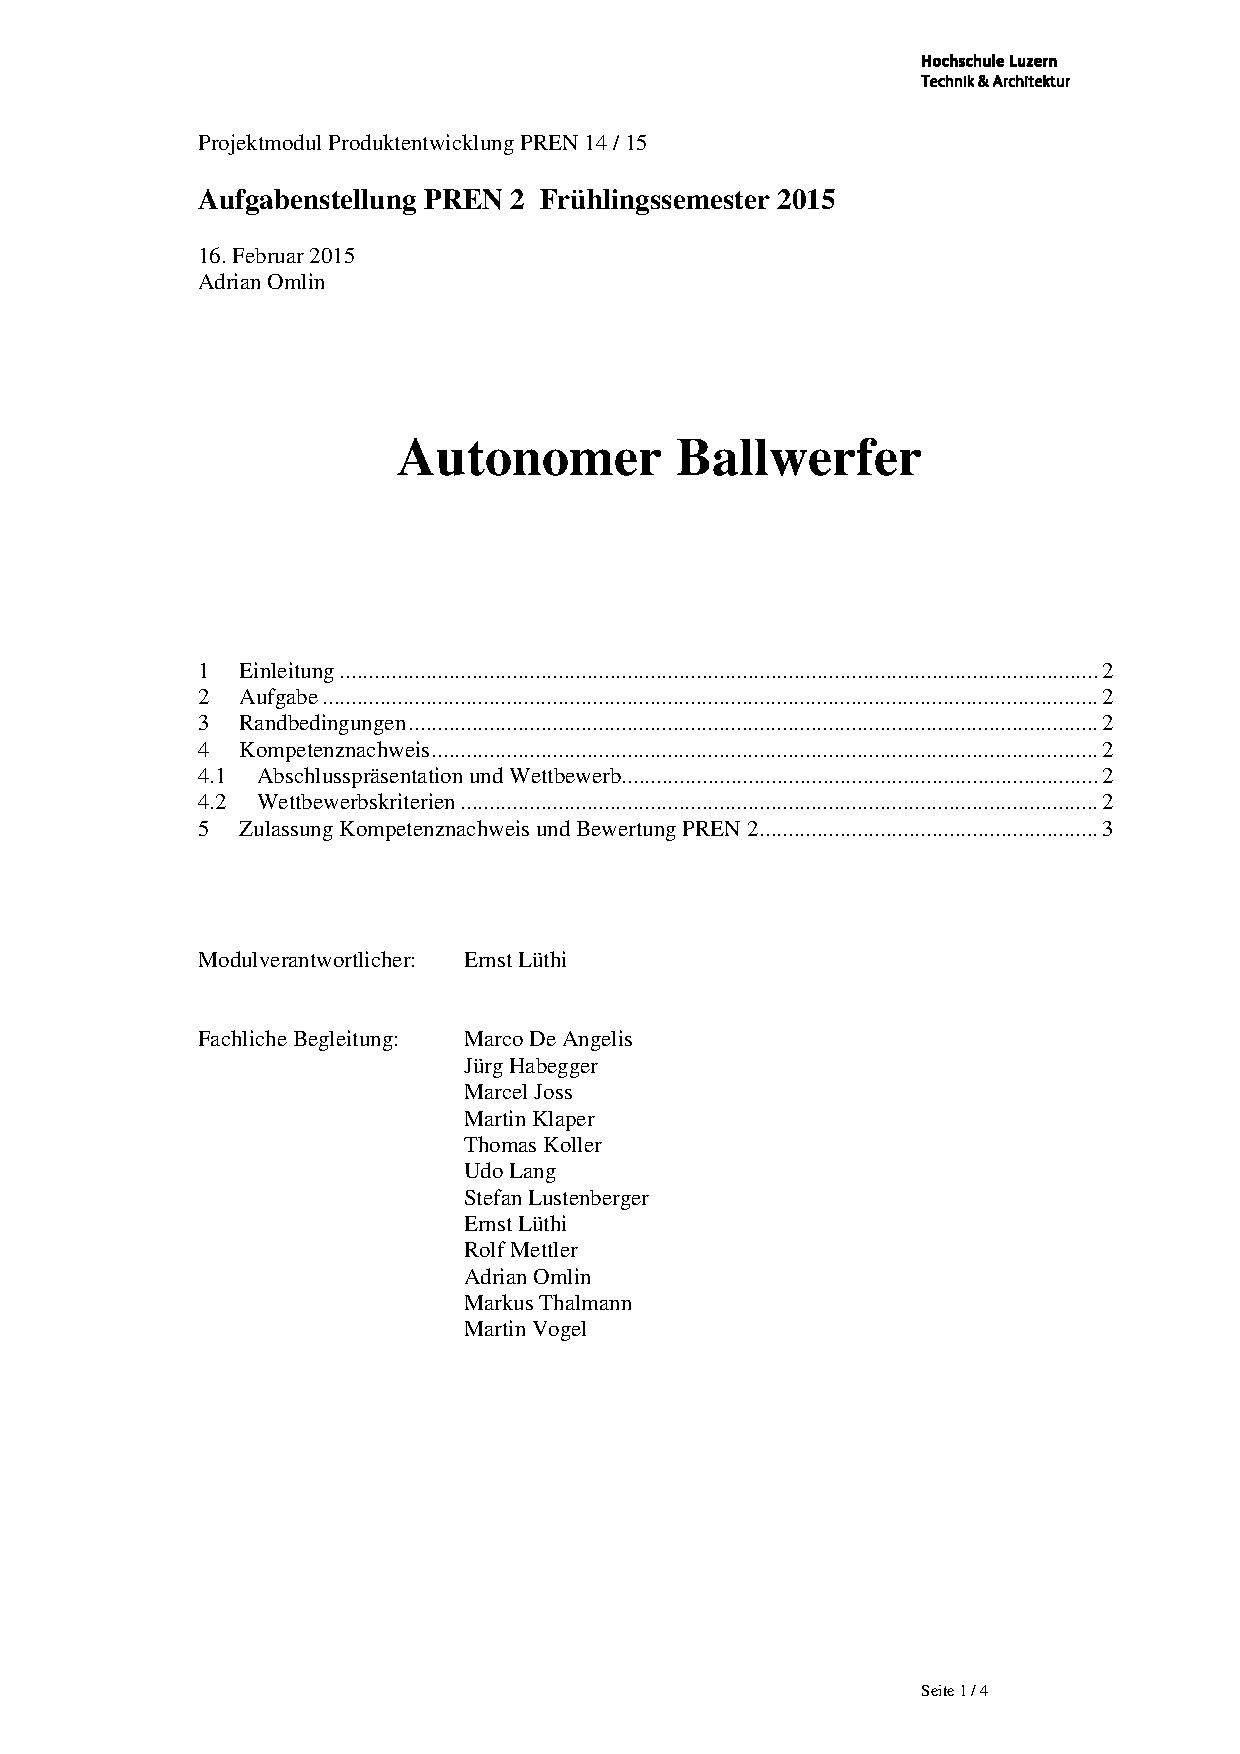
\includepdf[pages=-,offset=0 -2.2cm,frame,width=0.92\textwidth,picturecommand={\centering},pagecommand={\thispagestyle{fancy}},]{../../fig/Aufgabenstellung_PREN2_F15.pdf}
\newpage
\section{Technologierecherche}


\includepdf[pages=-,offset=0 -2.2cm,frame,width=0.92\textwidth,picturecommand={\centering},pagecommand={\thispagestyle{fancy}},]{../../fig/Team_39_Technologierecherche.pdf}
\newpage
\section{Produktanforderungen}
\label{sec:produktanforderungen}

Die Anforderungen wurden vom Team im PREN1 definiert und durch den betreuenden Dozenten abgenommen. Im Verlaufe des PREN2 wurden die Anforderungen angepasst und durch den Dozenten bestätigt. Nachfolgend liegt die vollständige Anforderungsliste vor. Auf der Liste ist erkennbar, welche Anforderungen geändert wurden. Nicht mehr gültige Anforderungen sind \sout{durchstrichen} und neue Elemente sind \uline{unterstrichen}.

\renewcommand{\arraystretch}{1.5}
\begin{longtable}[l]{|l|c|l|p{8.5cm}|}
	\hline
	\textbf{Nr.} & \textbf{F/M/W} & \textbf{Bezeichnung} & \textbf{Wert/Daten/Erläuterungen} \endhead
	
	\hline 1 &  & Gerät & \\ 
	\hline 1.1 & F & Gerätemasse & 0.5 m $\times$ 0.5 m $\times$ 1.0 m  \\
	\hline 1.2 & M & Gewicht & < 8 kg (ohne Energieversorgung, Tennisbälle und externes Kommunikationsgerät) sonst 0 Punkt \\
	\hline 1.3 & W & Gewicht & \sout{< 4 kg} \newline \uline{< 6 kg (Begründung: Gewählter Aufbau wird durch Motoren und Konstruktion schwerer)} \\
	\hline 1.4 & W & Standfestigkeit & stabil \\
	\hline 1.5 & F & Startbefehl & drahtlos über ein externes Kommunikationsgerät (\sout{Smartphone}, \sout{Tablet}, Computer) \newline \uline{Es wird lediglich eine Java-Applikation für das Notebook entwickelt. Die Zeit ist zu knapp um ein App zu entwickeln.} \\   
	\hline 1.6 & F & Stoppbefehl & auf demselben Kommunikationsgerät \sout{akustisch oder} visuell ausgegeben \newline \uline{Akustisch ist keine Pflicht, wenn es visuell ausgegeben wird. Akustisch wird somit nicht benötigt.}  \\ 
	\hline 1.7 & W & Kommunikationsgerät & \sout{App auf Smartphone} \newline \uline{App keine Pflicht. Die Applikation läuft auf dem Notebook. Der Zeitraum um eine App zu entwickeln ist zu klein.} \\
	\hline 1.8 & F & Aufhängevorrichtung & muss vorhanden sein (Wägen) \\
	\hline 1.9 & F & Selbstständigkeit & keine Eingriffe von aussen nach dem Start \\
	\hline 1.10 & W & Trefferquote & 100 \% (5 von 5 Bällen) \\
	\hline 1.11 & W & Prozesszeit & \sout{< 1 Min}. \newline
	\uline{< 90 Sekunden. Nachdem erkannt wurde, dass die Bilderkennung auf dem Raspberry PI nicht so rasant ist wie auf dem Notebook, sind wir mit der Zeit von 90 Sekunden zufrieden. Wichtiger ist die Stabilität und Funktionstüchtigkeit des Systems.} \\
	\hline 1.12 & M & Startpositionierung & von Hand mithilfe von Schablone \\
	\hline 2 &  & Energieversorgung & \\
	\hline 2.1 & W & Bauart & einfach zu entnehmen  \\
	\hline 2.2 & F & Bereitstellung & muss transportierbar sein  \\
	\hline 2.3 & W & Wirkungsgrad & hoch \\
	\hline 3 &  & Spielfeld & \\
	\hline 3.1 & F & Abmasse & siehe Aufgabenstellung \\       
	\hline 3.2 & F & Spielfeldrand & darf nicht umgriffen werden  \\
	\hline 3.3 & F & Zone ohne Hindernisse & 0.5 m $\times$ 0.5 m $\times$ 1.8 m um Spielfeldrand \\
	\hline 3.4 & F & Veränderungen am Spielfeld & keine erlaubt (z.B. Führungsschiene) \\
	\hline 3.5 & F & Begrenzungslinie & darf nicht überragen oder überfahren werden \\
	\hline 3.6 & F & Spielfeldboden & besteht aus hellen Spanplatten \\
	\hline 3.7 & F & Spielfeldrückwand & besteht aus hellen Spanplatten \\
	\hline 4 &  & Tennisball & \\
	\hline 4.1 & F & Gewicht & 55 g - 60 g  \\
	\hline 4.2 & F & Durchmesser & 6.3 cm - 7.3 cm   \\
	\hline 4.3 & F & Farbe & gelb \\
	\hline 4.4 & F & Modifikationen & nicht erlaubt  \\
	\hline 5 &  & Korb & \\
	\hline 5.1 & F & Höhe & 40 cm $\pm$ 2 cm \\        
	\hline 5.2 & F & Durchmesser & > 30 cm  \\ 
	\hline 5.3 & F & Farbe & schwarz  \\
	\hline 5.4 & F & Befestigung & abgestützt an Rückwand  \\
	\hline 5.5 & F & Position & innerhalb des Positionierungsfeldes (siehe Aufgabenstellung) seitlich verschiebbar  \\   
	\hline 5.6 & F & Dämpfung & mit Sand oder Kissen damit Ball nicht rausspringt  \\
	\hline 5.7 & F & Positionierung des Korbes & wird kurz (3 Sek.) vor dem Start positioniert  \\
	\hline 6 &  & Wettbewerbskriterien & \\
	\hline 6.1 & F & Einrichtzeit & 5 Min. \\
	\hline 6.2 & F & Probewürfe & 2 Versuche \\    
	\hline 6.3 & F & Spielzeit & max. 5 Min. \\
	\hline 6.4 & F & Bewertungsformel & \textit{Anzahl Bälle + (5 [Min] - Spielzeit [Min])/[Min] + Gewichtspunkte}  \\  
	\hline 6.5 & F & Gewichtspunkte &
	\renewcommand{\arraystretch}{1.1} 
	\begin{tabular}{l l l l l l}
		&   & m & $\leq$ & 2 kg & 4 Punkte \\
		2 kg & < & m & $\leq$ & 4 kg & 3 Punkte \\
		4 kg & < & m & $\leq$ & 6 kg & 2 Punkte \\
		6 kg & < & m & $\leq$ & 8 kg & 1 Punkt  \\
		8 kg & < & m &        &      & 0 Punkte \\
	\end{tabular} \\
	\hline 6.6 & F & Trefferquote & min. 1 Ball im Korb sonst 0 Punkte \\
	\hline 7 &  & Kosten & \\
	\hline 7.1 & F & Budget & 600.- Fr. (200.- Fr. für PREN 1) \\
	\hline 7.2 & F & Normteil & von HSLU Werkstatt beziehen \\
	\hline 7.3 & F & Teile von Sponsoren & erlaubt (Kosten werden angerechnet) \\
	\hline 7.4 & F & externes Kommunikationsgerät & Kosten werden nicht angerechnet \\
	\hline 7.5 & F & externes Netzgerät & Kosten werden nicht angerechnet \\
	\hline 7.6 & F & Occasion Material & \textonehalf-Kosten werden angerechnet \\
	\hline 8 &  & Umgebungsbedingungen & \\
	\hline 8.1 & F & Temperatur & 15$^\circ$C - 40$^\circ$C \\
	\hline 8.2 & F & Luftfeuchtigkeit & 30 \% - 80 \% (nicht kondensierend) \\
	\hline 8.3 & F & Spielfeldoberfläche & trocken und rau \\
	\hline 8.4 & F & Unebenheiten auf Spielfeld & $\leq$ 1mm \\
	\hline 8.5 & F & Luft & klar \\
	\hline 8.6 & F & Licht & 1'200 lm - 100'000 lm (homogene Beleuchtung) \\
	\hline 8.7 & F & Spielfeldneigung & $\leq$ 2$^\circ$ \\
	\hline 8.8 & F & Standfestigkeit & stabil \\
	\hline 8.9 & F & Windgeschwindigkeit & $\leq$ 1m/s \\
	\hline 9 &  & Sicherheit & \\
	\hline 9.1 & M & Gefährdungspotential & gering für Anwender \\
	\hline 9.2 & M & Schutzart & IP20 \\
	\hline 9.3 & M & Schutzleiter & muss vorhanden sein \\
	\hline 10 &  & Recycling & \\
	\hline 10.1 & W & Trennung & unterschiedliche Werkstoffe einfach trennbar \\
	\hline 11 &  & Montage & \\
	\hline 11.1 & W & Komponenten & schnell und einfach montierbar/demontierbar \\
	\hline 11.2 & W & Spezialwerkezug & ohne Spezialwerkzeug montierbar/demontierbar \\
	\hline 
	
\end{longtable}
\newpage
%Funktionsanalyse, Lösungsansätze und Bewertungen
\input{content/funktion-loesung}
\newpage
\input{content/detaillierte-berechnungen}
\newpage
%Versuche und Tests: Testplanung, Details, Messprotokolle etc.
\input{content/versuche-tests-anhang}
\newpage
%Meilensteinberichte, Protokolle, Pendenzenlisten
\input{content/berichte}
\newpage

\section{Anforderungen}

Die Anforderungen wurden vom Team im PREN1 definiert und durch den betreuenden Dozenten abgenommen. Im Verlaufe des PREN2 wurden die Anforderungen angepasst und durch den Dozenten bestätigt. Nachfolgend liegt die vollständige Anforderungsliste vor. Auf der Liste ist erkennbar, welche Anforderungen geändert wurden. Nicht mehr gültige Anforderungen sind \sout{durchstrichen} und neue Elemente sind \uline{unterstrichen}.

\begin{longtable}[l]{|l|c|l|p{8.5cm}|}
	\hline
	\textbf{Nr.} & \textbf{F/M/W} & \textbf{Bezeichnung} & \textbf{Wert/Daten/Erläuterungen} \endhead
	
	\hline 1 &  & Gerät & \\ 
	\hline 1.1 & F & Gerätemasse & 0.5 m $\times$ 0.5 m $\times$ 1.0 m  \\
	\hline 1.2 & M & Gewicht & < 8 kg (ohne Energieversorgung, Tennisbälle und externes Kommunikationsgerät) sonst 0 Punkt \\
	\hline 1.3 & W & Gewicht & \sout{< 4 kg} \newline \uline{< 6 kg (Begründung: Gewählter Aufbau wird durch Motoren und Konstruktion schwerer)} \\
	\hline 1.4 & W & Standfestigkeit & stabil \\
	\hline 1.5 & F & Startbefehl & drahtlos über ein externes Kommunikationsgerät (\sout{Smartphone}, \sout{Tablet}, Computer) \newline \uline{Es wird lediglich eine Java-Applikation für das Notebook entwickelt. Die Zeit ist zu knapp um ein App zu entwickeln.} \\   
	\hline 1.6 & F & Stoppbefehl & auf demselben Kommunikationsgerät \sout{akustisch oder} visuell ausgegeben \newline \uline{Akustisch ist keine Pflicht, wenn es visuell ausgegeben wird. Akustisch wird somit nicht benötigt.}  \\ 
	\hline 1.7 & W & Kommunikationsgerät & \sout{App auf Smartphone} \newline \uline{App keine Pflicht. Die Applikation läuft auf dem Notebook. Der Zeitraum um eine App zu entwickeln ist zu klein.} \\
	\hline 1.8 & F & Aufhängevorrichtung & muss vorhanden sein (Wägen) \\
	\hline 1.9 & F & Selbstständigkeit & keine Eingriffe von aussen nach dem Start \\
	\hline 1.10 & W & Trefferquote & 100 \% (5 von 5 Bällen) \\
	\hline 1.11 & W & Prozesszeit & \sout{< 1 Min}. \newline
	\uline{< 90 Sekunden. Nachdem erkannt wurde, dass die Bilderkennung auf dem Raspberry PI nicht so rasant ist wie auf dem Notebook, sind wir mit der Zeit von 90 Sekunden zufrieden. Wichtiger ist die Stabilität und Funktionstüchtigkeit des Systems.} \\
	\hline 1.12 & M & Startpositionierung & von Hand mithilfe von Schablone \\
	\hline 2 &  & Energieversorgung & \\
	\hline 2.1 & W & Bauart & einfach zu entnehmen  \\
	\hline 2.2 & F & Bereitstellung & muss transportierbar sein  \\
	\hline 2.3 & W & Wirkungsgrad & hoch \\
	\hline 3 &  & Spielfeld & \\
	\hline 3.1 & F & Abmasse & siehe Aufgabenstellung \\       
	\hline 3.2 & F & Spielfeldrand & darf nicht umgriffen werden  \\
	\hline 3.3 & F & Zone ohne Hindernisse & 0.5 m $\times$ 0.5 m $\times$ 1.8 m um Spielfeldrand \\
	\hline 3.4 & F & Veränderungen am Spielfeld & keine erlaubt (z.B. Führungsschiene) \\
	\hline 3.5 & F & Begrenzungslinie & darf nicht überragen oder überfahren werden \\
	\hline 3.6 & F & Spielfeldboden & besteht aus hellen Spanplatten \\
	\hline 3.7 & F & Spielfeldrückwand & besteht aus hellen Spanplatten \\
	\hline 4 &  & Tennisball & \\
	\hline 4.1 & F & Gewicht & 55 g - 60 g  \\
	\hline 4.2 & F & Durchmesser & 6.3 cm - 7.3 cm   \\
	\hline 4.3 & F & Farbe & gelb \\
	\hline 4.4 & F & Modifikationen & nicht erlaubt  \\
	\hline 5 &  & Korb & \\
	\hline 5.1 & F & Höhe & 40 cm $\pm$ 2 cm \\        
	\hline 5.2 & F & Durchmesser & > 30 cm  \\ 
	\hline 5.3 & F & Farbe & schwarz  \\
	\hline 5.4 & F & Befestigung & abgestützt an Rückwand  \\
	\hline 5.5 & F & Position & innerhalb des Positionierungsfeldes (siehe Aufgabenstellung) seitlich verschiebbar  \\   
	\hline 5.6 & F & Dämpfung & mit Sand oder Kissen damit Ball nicht rausspringt  \\
	\hline 5.7 & F & Positionierung des Korbes & wird kurz (3 Sek.) vor dem Start positioniert  \\
	\hline 6 &  & Wettbewerbskriterien & \\
	\hline 6.1 & F & Einrichtzeit & 5 Min. \\
	\hline 6.2 & F & Probewürfe & 2 Versuche \\    
	\hline 6.3 & F & Spielzeit & max. 5 Min. \\
	\hline 6.4 & F & Bewertungsformel & \textit{Anzahl Bälle + (5 [Min] - Spielzeit [Min])/[Min] + Gewichtspunkte}  \\  
	\hline 6.5 & F & Gewichtspunkte &
	\renewcommand{\arraystretch}{1.1} 
	\begin{tabular}{l l l l l l}
		&   & m & $\leq$ & 2 kg & 4 Punkte \\
		2 kg & < & m & $\leq$ & 4 kg & 3 Punkte \\
		4 kg & < & m & $\leq$ & 6 kg & 2 Punkte \\
		6 kg & < & m & $\leq$ & 8 kg & 1 Punkt  \\
		8 kg & < & m &        &      & 0 Punkte \\
	\end{tabular} \\
	\hline 6.6 & F & Trefferquote & min. 1 Ball im Korb sonst 0 Punkte \\
	\hline 7 &  & Kosten & \\
	\hline 7.1 & F & Budget & 600.- Fr. (200.- Fr. für PREN 1) \\
	\hline 7.2 & F & Normteil & von HSLU Werkstatt beziehen \\
	\hline 7.3 & F & Teile von Sponsoren & erlaubt (Kosten werden angerechnet) \\
	\hline 7.4 & F & externes Kommunikationsgerät & Kosten werden nicht angerechnet \\
	\hline 7.5 & F & externes Netzgerät & Kosten werden nicht angerechnet \\
	\hline 7.6 & F & Occasion Material & \textonehalf-Kosten werden angerechnet \\
	\hline 8 &  & Umgebungsbedingungen & \\
	\hline 8.1 & F & Temperatur & 15$^\circ$C - 40$^\circ$C \\
	\hline 8.2 & F & Luftfeuchtigkeit & 30 \% - 80 \% (nicht kondensierend) \\
	\hline 8.3 & F & Spielfeldoberfläche & trocken und rau \\
	\hline 8.4 & F & Unebenheiten auf Spielfeld & $\leq$ 1mm \\
	\hline 8.5 & F & Luft & klar \\
	\hline 8.6 & F & Licht & 1'200 lm - 100'000 lm (homogene Beleuchtung) \\
	\hline 8.7 & F & Spielfeldneigung & $\leq$ 2$^\circ$ \\
	\hline 8.8 & F & Standfestigkeit & stabil \\
	\hline 8.9 & F & Windgeschwindigkeit & $\leq$ 1m/s \\
	\hline 9 &  & Sicherheit & \\
	\hline 9.1 & M & Gefährdungspotential & gering für Anwender \\
	\hline 9.2 & M & Schutzart & IP20 \\
	\hline 9.3 & M & Schutzleiter & muss vorhanden sein \\
	\hline 10 &  & Recycling & \\
	\hline 10.1 & W & Trennung & unterschiedliche Werkstoffe einfach trennbar \\
	\hline 11 &  & Montage & \\
	\hline 11.1 & W & Komponenten & schnell und einfach montierbar/demontierbar \\
	\hline 11.2 & W & Spezialwerkezug & ohne Spezialwerkzeug montierbar/demontierbar \\
	\hline 
	
\end{longtable}
\newpage
\section{Schnittstellen}

\section{REST von Webserver}

Die Schnittstelle von der externen Steuereinheit zum Raspberry Pi wird über eine REST\footnote{Representational State Transfer}-Schnittstelle realisiert. Es wurden folgende Ressourcen definiert:
\begin{itemize}
	\item camera
	\item image
	\item start
\end{itemize}
Jede Ressource lässt sich mit HTML-Methoden (GET, PUT, POST usw.) abrufen oder verändern. Die Schnittstelle lässt sich ohne Authentifizierung nutzen und arbeiten mit dem JSON-Datenformat. Nachfolgend werden die einzelnen Ressourcen näher beschrieben.

\subsection{GET camera}

Diese Anfrage liefert die aktuellen Einstellungen der Bilderkennung zurück.

\subsubsection{Parameter}

\begin{tabular}{l p{16cm}}
	\textbf{config} & Die Konfiguration der Bilderkennung \\
	\textbf{roi} & Ist der Bereich in dem der Korb erkennbar ist (Region of Interest). Er ist definiert durch die Koordinaten der linken oberen Ecke (x,y) und einer Fläche (height, width). \\
	\textbf{contrast} & Ein Wert zwischen -100 und 100 für den Kontrast der Kamera. \\
	\textbf{greyscale} & \texttt{true} wenn ein Graustufen-Bild erzeugt werden soll. \\
	\textbf{quality} & Ein Wert zwischen 0 und 100 für die Qualität des JPEG-Bildes. \\
	\textbf{line} & Die Pixellinie welche analysiert werden soll um den Korb zu detektieren. \\
	\textbf{height} & Auf welcher Höhe soll die Pixellinie analysiert werden. Darf max. so hoch sein wie die ROI. \\
	\textbf{area} & Bei der Detektierung wird nicht nur eine Pixellinie untersucht. Mit \texttt{area} kann ein Band definiert werden in dem die Linien analysiert werden. \\
	\textbf{image} & Der URL zum Bild der Kamera. Bei jedem Aufruf wird ein neues Bild erstellt.
\end{tabular}

\subsubsection{Beispiel Request}

\texttt{GET} \\
\texttt{http://<raspberrypi-ip>/camera}

\subsubsection{Beispiel Result}

\begin{lstlisting}[caption=GET camera Result, label=lst:camera, tabsize=2]
{
	"config": {
		"roi": {
			"x": 100,
			"y": 200,
			"height": 300,
			"width": 400
		},
		"contrast": 50,
		"greyscale": true,
		"quality": 100,
		"line": {
			"height": 300,
			"area": 5
		}
	},
	"image": "http://<raspberrypi-ip>/image"
}
\end{lstlisting}

\subsection{PUT camera}

Diese Anfrage verändert die Einstellungen der Bilderkennung.

\subsubsection{Beispiel Request}

\texttt{PUT} \\
\texttt{http://<raspberrypi-ip>/camera} \\
Body siehe Listing \ref{lst:camera}

\subsubsection{Beispiel Result}

\begin{lstlisting}[caption=PUT camera Result, tabsize=2]
{
	"status": true
}
\end{lstlisting}

\subsection{GET image}

Diese Anfrage liefert das Bild der Kamera zurück. Bei jeder Anfrage wird ein Bild erstellt.

\subsubsection{Beispiel Request}

\texttt{GET} \\
\texttt{http://<raspberrypi-ip>/image}

\subsubsection{Beispiel Result}

Bild im JPEG-Format

\subsection{GET start}

Diese Anfrage liefert den Status des Vorgangs zurück. Wenn \texttt{start} auf \texttt{true} gesetzt ist läuft der Vorgang.

\subsubsection{Beispiel Request}

\texttt{GET} \\
\texttt{http://<raspberrypi-ip>/start}

\subsubsection{Beispiel Result}

\begin{lstlisting}[caption=GET start Result, tabsize=2]
{
	"start": true
}
\end{lstlisting}

\subsection{PUT start}

Diese Anfrage startet den Vorgang und übergibt die Callback-Adresse vom Steuergerät, damit der Stopp-Befehl zurück gesendet werden kann.

\subsubsection{Parameter}

\begin{tabular}{l p{16cm}}
	\textbf{start} & Bei \texttt{true} wird der Vorgang gestartet. Der Vorgang wird nicht unterbrochen falls \texttt{start} auf \texttt{false} gesetzt wird. Ist der Vorgang beendet wird \texttt{start} auf \texttt{false} gesetzt \\
	\textbf{url} & Die IP-Adresse des Steuergerätes. Diese wird benötigt um den Stopp-Befehl zurückzusenden.
\end{tabular}

\subsubsection{Beispiel Request}

\texttt{PUT} \\
\texttt{http://<raspberrypi-ip>/start}

\begin{lstlisting}[caption=PUT start Request, tabsize=2]
{
	"start": true,
	"url": "http://<steuergerät-ip>"
}
\end{lstlisting}

\subsubsection{Beispiel Result}

\begin{lstlisting}[caption=PUT start Result, tabsize=2]
{
	"status": true
}
\end{lstlisting}
\newpage
\section{Testplan}
Es wird zwischen Integrations- (INT) und Systemtest (SYS) unterschieden. Ein Integrationstest
ist technisch getrieben und prüft das Zusammenspiel der Komponenten. Aus diesem
Grund wird empfohlen, dass solche Tests von den Entwicklern selber durchgeführt werden.
Systemtest hingegen sind benutzerorientiert. Diese testen das System als Ganzes.
Die Tests sind voneinander abhängig, darum ist die Reihenfolge der Testausführung
definiert. Denn ein Test kann als Vorbedingung für einen anderen Test gelten. 

In den Tests wird von Controller und Configurator gesprochen. Der Controller ist
das Raspberry Pi und der Configurator die externe Steuerungseinheit.

\subsection{Reihenfolge der Testdurchführung}
INT101, INT102, INT103, INT104
SYS101, SYS102, SYS103, SYS104

\subsection{INT101 Webservice Erreichbarkeit}
\begin{table}[h!]
	\renewcommand{\arraystretch}{1.5}
	\begin{tabular}{|r|p{14cm}|}
		\hline Beschreibung & Die Webservices auf dem Controller müssen erreichbar sein. \\ 
		\hline Vorbedingungen & Controller Setup \\ 
		\hline Testdaten & URL: http://<IP_ADDRESS_CONTROLLER>:<PORT_CONTROLLER> \\ 
		\hline Vorgehen & 
		\begin{enumerate}
			\item Browser öffnen und URL eingeben.
		\end{enumerate} \\ 
		\hline Ergebnis & Der Browser zeigt eine Willkommensseite an \\ 
		\hline 
	\end{tabular}
\end{table}

\subsection{INT102 Webservice Bild laden}
\begin{table}[h!]
	\renewcommand{\arraystretch}{1.5}
	\begin{tabular}{|r|p{14cm}|}
		\hline Beschreibung & Der Bild-Lade Webservice muss ein Bild zurückliefern. \\ 
		\hline Vorbedingungen & INT101 \\ 
		\hline Testdaten & URL: http://<IP_ADDRESS_CONTROLLER>:<PORT_CONTROLLER>/image \\ 
		\hline Vorgehen & 
		\begin{enumerate}
			\item Browser öffnen und URL eingeben
		\end{enumerate} \\ 
		\hline Ergebnis & Ein Bild wird angezeigt. \\ 
		\hline 
	\end{tabular}
\end{table}

\subsection{INT103 Webservice Kamera Konfig laden}
\begin{table}[h!]
	\renewcommand{\arraystretch}{1.5}
	\begin{tabular}{|r|p{14cm}|}
		\hline Beschreibung & Der Kamera-Konfig-Lade Webservice muss ein JSON-File mit den aktuellen Einstellungen liefern. \\ 
		\hline Vorbedingungen & INT102 \\ 
		\hline Testdaten & URL: http://<IP_ADDRESS_CONTROLLER>:<PORT_CONTROLLER>/camera \\ 
		\hline Vorgehen & 
		\begin{enumerate}
			\item Browser öffnen und URL eingeben
		\end{enumerate} \\ 
		\hline Ergebnis & JSON-File mit aktuellen Einstellungen ist ersichtlich. \\ 
		\hline 
	\end{tabular}
\end{table}

\subsection{INT104 Webservice Kamera Konfig speichern}
\begin{table}[h!]
	\renewcommand{\arraystretch}{1.5}
	\begin{tabular}{|r|p{14cm}|}
		\hline Beschreibung & Der Kamera-Konfig-Speicher Webservice muss ein JSON-File entgegennehmen und die Einstellungen speichern. \\ 
		\hline Vorbedingungen & INT103 \\ 
		\hline Testdaten & URL: http://<IP_ADDRESS_CONTROLLER>:<PORT_CONTROLLER>/camera \\ 
		\hline Vorgehen & 
		\begin{enumerate}
			\item Aktuelle Controller Einstellungen laden.
			\item Einstellungen in ein JSON-File speichern.
			\item Ein paar Werte anpassen.
			\item PUT Request an die URL senden mit dem JSON-File.
			\item Controller neu starten
			\item Aktuelle Controller Einstellungen laden.
		\end{enumerate} \\ 
		\hline Ergebnis & Die Einstellungen müssen nun die gleichen sein wie vor dem Neustart. \\ 
		\hline 
	\end{tabular}
\end{table}

\subsection{SYS101 Configurator startet}
\begin{table}[h!]
	\renewcommand{\arraystretch}{1.5}
	\begin{tabular}{|r|p{14cm}|}
		\hline Beschreibung & Der Configurator lässt sich starten. \\ 
		\hline Vorbedingungen & Configurator Setup \\ 
		\hline Testdaten &  \\ 
		\hline Vorgehen & 
		\begin{enumerate}
			\item Configurator starten
		\end{enumerate} \\ 
		\hline Ergebnis & Es erscheint eine Benutzeroberfläche. \\ 
		\hline 
	\end{tabular}
\end{table}

\subsection{SYS102 Configurator Verbindungseinstellungen }
\begin{table}[h!]
	\renewcommand{\arraystretch}{1.5}
	\begin{tabular}{|r|p{14cm}|}
		\hline Beschreibung & Im Configurator lassen sich die Verbindungseinstellungen zum Controller ändern. \\ 
		\hline Vorbedingungen & SYS101 \\ 
		\hline Testdaten & Eigene Verbindungsdaten definieren \\ 
		\hline Vorgehen & 
		\begin{enumerate}
			\item Configurator starten
			\item Verbindungeinstellungen ändern und speichern
			\item Configurator neu starten
		\end{enumerate} \\ 
		\hline Ergebnis & Verbindungseinstellungen sind auch nach dem Neustart erhalten. \\ 
		\hline 
	\end{tabular}
\end{table}

\subsection{SYS103 Configurator Bild laden }
\begin{table}[h!]
	\renewcommand{\arraystretch}{1.5}
	\begin{tabular}{|r|p{14cm}|}
		\hline Beschreibung & Aktuelle Foto lässt sich laden und im Configurator anzeigen. \\ 
		\hline Vorbedingungen & SYS102 \\ 
		\hline Testdaten & Verbindungsdaten definieren, Bild \\ 
		\hline Vorgehen & 
		\begin{enumerate}
			\item Configurator starten
			\item Bild laden
		\end{enumerate} \\ 
		\hline Ergebnis & Aktuelles Foto erscheint im GUI. Auf dem Bild muss der Korb markiert sein und der Winkel angegeben. \\ 
		\hline 
	\end{tabular}
\end{table}

\subsection{SYS104 Configurator Konfiguration anwenden }
\begin{table}[h!]
	\renewcommand{\arraystretch}{1.5}
	\begin{tabular}{|r|p{14cm}|}
		\hline Beschreibung & Die Kamera-Einstellungen lassen sich editieren und auf den Controller anwenden. \\ 
		\hline Vorbedingungen & SYS103 \\ 
		\hline Testdaten & Konfigurationsdaten \\ 
		\hline Vorgehen & 
		\begin{enumerate}
			\item Configurator starten
			\item Kamera-Einstellunge editieren
			\item Kamera-Einstellung speichern
			\item Bild neu laden
		\end{enumerate} \\ 
		\hline Ergebnis & Auf dem GUI erscheint die Meldung, dass die Konfiguration erfolgreich gespeichert wurde.
		Ausserdem erscheint das Bild, welches mit den aktuellen Einstellungen modifiziert wurden. \\ 
		\hline 
	\end{tabular}
\end{table}
\newpage
\section{Testprotokoll}

\subsection{Zusammenfassung}

\begin{table}[h!]
	\centering
	\renewcommand{\arraystretch}{1.5}
	\begin{tabular}{|c|c|c|c|c|}
		\hline \textbf{Tester} & \textbf{Datum} & \textbf{Anzahl Tests} & \textbf{Tests erfolgreich} & \textbf{Tests fehlgeschlagen} \\
		\hline Adrian Würsch & 29.05.2015 & 31 & 31 & 0 \\ 
		\hline 
	\end{tabular}
\end{table}

\subsection{Versionen}

\begin{table}[h!]
	\centering
	\renewcommand{\arraystretch}{1.5}
	\begin{tabular}{|l|l|}
		\hline \textbf{Komponente} & \textbf{Version} \\
		\hline Webserver & v0.0.1 \\
		\hline Drives & v0.0.1 \\
		\hline Detection & v0.0.1 \\
		\hline Camera & v0.0.1 \\
		\hline 
	\end{tabular}
\end{table}

\newpage
\subsection{Testergebnisse}

\begin{table}[h!]
	\centering
	\renewcommand{\arraystretch}{1.5}
	\begin{tabular}{|l|c|p{8cm}|}
		\hline \textbf{Test} & \textbf{IO/NIO} & \textbf{Bemerkungen} \\
		\hline GST101 Ballwerfer ausgerichtet & IO & \\
		\hline GST102 Strom angeschlossen & IO & \\
		\hline GST103 Boards eingeschaltet & IO & \\
		\hline GST104 Verbindung aufgebaut & IO & \\
		\hline GST105 GUI geöffnet & IO & \\
		\hline GST106 Reset Motoren & IO & \\
		\hline GST107 Bälle eingefüllt & IO & \\
		\hline GST108 Kamera kalibriert & IO & \\
		\hline MB101 Funktionskontrolle Schrittmotor & IO & \\
		\hline MB102 Funktionskontrolle DC-Motor & IO & \\
		\hline MB103 Funktionskontrolle BLDC-Motor & IO & \\
		\hline MB104 Stabilität Aufbau & IO & \\
		\hline MB105 Funktionskontrolle Treffgenauigkeit & IO & \\
		\hline KOM101 Kommunikation mit PC & IO & \\
		\hline KOM102 Kommunikation mit RaspberryPi & IO & \\
		\hline MOT101 Ballabwurf mit BLDC Motor & IO & \\
		\hline MOT102 Ballnachschub mit DC Motor & IO & \\
		\hline MOT103 Turmausrichtung mit Schrittmotor & IO & \\
		\hline POW101 Leistungsspeisung per Server-Netzteil & IO & \\
		\hline SEN101 Positionsschalter & IO & \\
		\hline INT101 Webservice Erreichbarkeit & IO & \\
		\hline INT102 Webservice Bild laden & IO & \\
		\hline INT103 Webservice Kamera Konfig laden & IO & \\
		\hline INT104 Webservice Kamera Konfig speichern & IO & \\
		\hline SYS101 Configurator startet & IO & \\
		\hline SYS102 Configurator Verbindungseinstellungen & IO & \\
		\hline SYS103 Configurator Bild laden & IO & \\
		\hline SYS104 Configurator Bild Konfiguration anwenden & IO & \\
		\hline SYS105 BLDC ansteuern & IO & \\
		\hline SYS106 DC ansteuern & IO & \\
		\hline SYS107 STP ansteuern & IO & \\
		\hline 
	\end{tabular}
\end{table}


\begin{multicols}{2}
	\printglossary[title=Glossar,toctitle=Terms and abbreviations]
\end{multicols}
